
%Copyright (C) 2016 by Krishneel@JSK Lab, The University of Tokyo

%Copyright (C) 2016 by Krishneel@JSK Lab, The University of Tokyo

\documentclass{standalone}
\usepackage{footnote}
\usepackage{hyperref}
\usepackage{graphicx}
\usepackage{fancyhdr}

\renewcommand\footnoterule{%
  \kern-3\p@
  \hrule\@width2.5cm
  \kern2.6\p@
}
\makeatother

\begin{document}

\section{Software}


\subsection{Software Environment}
The motion planning and visual perception algorithms are implemented
on Robot Operating System (ROS) environment\footnote{\url{http://www.ros.org}}.
We used Gazebo\footnote{\url{gazebosim.org}} for virtual simulations
\footnote{\url{https://github.com/start-jsk/jsk_mbzirc}}. Our
algorithms are implemented in C/C++, Python and CUDA-C.


\subsection{Visual Perception}

The image processing is one of the fundamental component of autonomous
systems. With efficient and robust image processing the planning and
decision making can be done more readily which improves the accuracy
and robustness of executing the assigned task. Hence, one of our
primary objective while designing our software architectures was
real-time performance with minimal loss of accuracy. The visual
components of task one include three main stages described as follows:

\subsubsection{Target Detection}
The target detection phase is the initial localization of the landing
region (heliport) on the truck. To detect the heliport we use the
traditional computer vision detection approach where by a sliding
window based method is used. However such raster scanning windows are
computationally expensive even for high end systems. To overcome this
crucial limitation we first generate candidate objectness
regions. Since the heliport is fixed to a moving target, we use
Gaussian based background subtractor fused with Kalman Filters for 
global motion compensation to generate regions of interest
(ROI)  with stable changes. The candidate ROI's are then ranked using
edge similarity between each sliding window. High scoring ROI are then
used for detecting the heliport using pretrained detector. 
Let $\mathbf{H}$ denote the detected target region.

\subsubsection{Target Tracking}

In order for an UAV to approach and land on the heliport online visual
feedback is very important given that the target is constantly moving.
Using the assumption that the target is not
expected to change abruptly both in terms of visual motion and
appearances, we use visual tracking for online feedback.
The detected region $\mathbf{H}$ is used to initialize the
tracker. Our visual tracking algorithm is highly efficient and robust
to both scale and visual changes and runs in real time, thus
providing frame by frame location of the target. To enable a tracker
to run online in real time we carefully crafted the expensive process
of feature computation by reducing it to one time process. 
The invariant features for tracking are computed by passing the image
through several pre-trained kernels of varying dimensions. By varying
the sizes of the kernel, an approximate scale can also be detected.
Moreover, the tracker is updated online at fixed intervals.

\begin{figure}[t!]
  \centering
  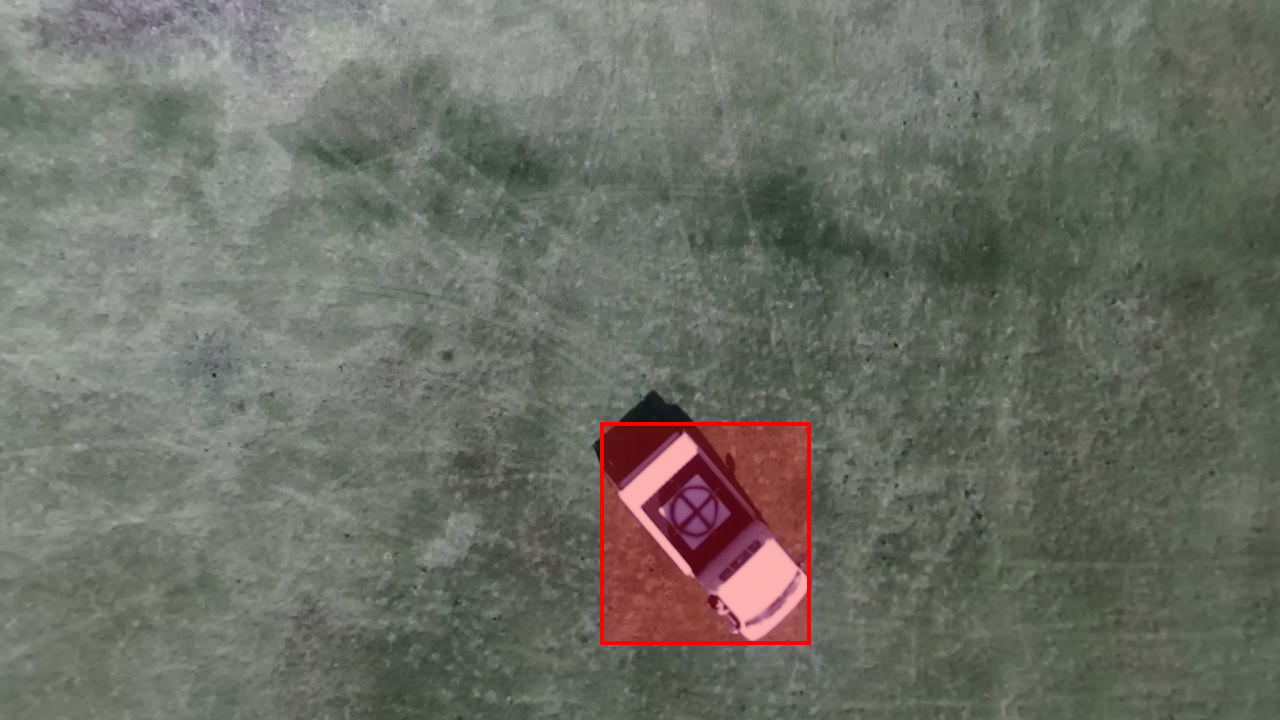
\includegraphics[height=1in]{sections/task1/images/detect2}
  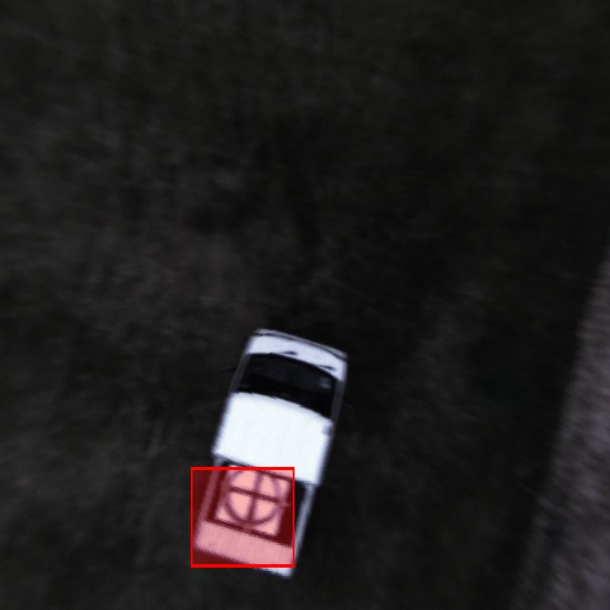
\includegraphics[height=1in]{sections/task1/images/detect1}
  \caption{Illustration of truck and heliport detection.}
\end{figure}

\subsection{Results Achieved to Date}

We have completed task one fully autonomously landing on the moving
target at 5km/h, 10km/h and 15km/h. The results of these landings are
shown in video. Moreover we demonstrate the effectiveness of our real
time planning and tracking by showing the results of long time
following of the target at over 35km/h. 

\end{document}
